\documentclass{beamer}

%\usetheme{Boxes}

\usepackage[utf8]{inputenc}
\usepackage[british,english]{babel}
\usepackage{verbatim}
\usepackage{graphicx}
\usepackage{colortbl}
\usepackage{color}
\usepackage{hyperref}
\usepackage{verbatim}
\usepackage{url}
\usepackage{moreverb}
\usepackage{fancyvrb}
%\usepackage{minted}
%\usepackage{algpseudocode}
%\usepackage{natbib}
%\usepackage{eulervm}
%\usepackage{auto-pst-pdf}
%\usepackage{pst-plot}
\usepackage{multirow}
\usepackage{subfigure}
\usepackage{arydshln}
\usepackage{multicol}

\hypersetup{colorlinks=true, linkcolor=black, urlcolor=blue}
\usetheme{boxes}
\beamertemplatenavigationsymbolsempty
\setbeamertemplate{sections/subsections in toc}[circle]
\setbeamertemplate{footline}[frame number]
\setbeamertemplate{itemize items}[circle]
\setbeamertemplate{itemize subitem}[square]

\title{{\bf Leveraging user-interaction and auxiliary data to learn from small data}}
\author{Romain Mormont}
\institute{Systems and modeling unit, \\
Department of EE \& CS, \\ University of Liège, Belgium}
\date{28th October 2016}  

\newcommand{\todo}[1]{\textcolor{red}{[TODO] #1}}

\definecolor{lightgreen}{rgb}{0.0,0.8,0.0}
\definecolor{lightblue}{rgb}{0.3,0.8,1.0}
\definecolor{lightred}{rgb}{0.874,0.180,0.105}
\definecolor{gray}{rgb}{0.4,0.4,0.4}
\definecolor{lightgray}{rgb}{0.8,0.8,0.8}
\definecolor{shadecolor}{rgb}{0.9,0.9,0.9}
%\newrgbcolor{mygreen}{.00 .5 .00}
%\newrgbcolor{myyellow}{.6 .6 .00}



%\newrgbcolor{mygreen}{.00 .5 .00}
%\newcommand{\X}[1]{\textcolor{blue}{#1}}
%\newcommand{\y}[1]{\textcolor{red}{#1}}
%\newcommand{\model}[1]{\textcolor{mygreen}{#1}}
%\newcommand{\loss}[1]{\textcolor{lightblue}{#1}}

\begin{document}
\setbeamertemplate{caption}{\raggedright\insertcaption\par}
\renewcommand{\inserttotalframenumber}{11}

% Title page ==================================================================

\begin{frame}
\titlepage
\end{frame}


\begin{frame}{Context}
	\begin{itemize}
		\item Supervised \textbf{machine learning} (ML) is about learning input-output models from data 
		\item It has recently gained popularity through several successes with important media coverage
		\item Those were mostly possible thanks to: 
		\begin{itemize}
			\item \textbf{Plenty of data} (\textit{big data})
			\item High computational power
		\end{itemize}
		\item Those criteria are essential to get the best performance out of common ML methods
	\end{itemize}
\end{frame}

\begin{frame}{Problem}
	\begin{itemize}
		\item \textbf{In practice, those two criteria are not always met}.
		\item Especially, data can be scarce. One can then talk about \textbf{small data} ! 
	\end{itemize}
	\vfill
	\begin{center}
		\large
		\textbf{Small data}: "the amount of data is not large enough with respect to the complexity of the task at hands" 
	\end{center}
	\vfill
	\begin{center}
		\small
		N.B.: in \textit{small data} settings, the amount of data is not necessarily small in absolute terms 
	\end{center}
\end{frame}


\begin{frame}{Case study}
	\begin{center}
		\textbf{Rare object detection and categorization in high-resolution tissue images}.
	\end{center}
		
	\begin{figure}[h]
		\center
		\caption{Thyroid nodule malignancy diagnosis}
		\subfigure{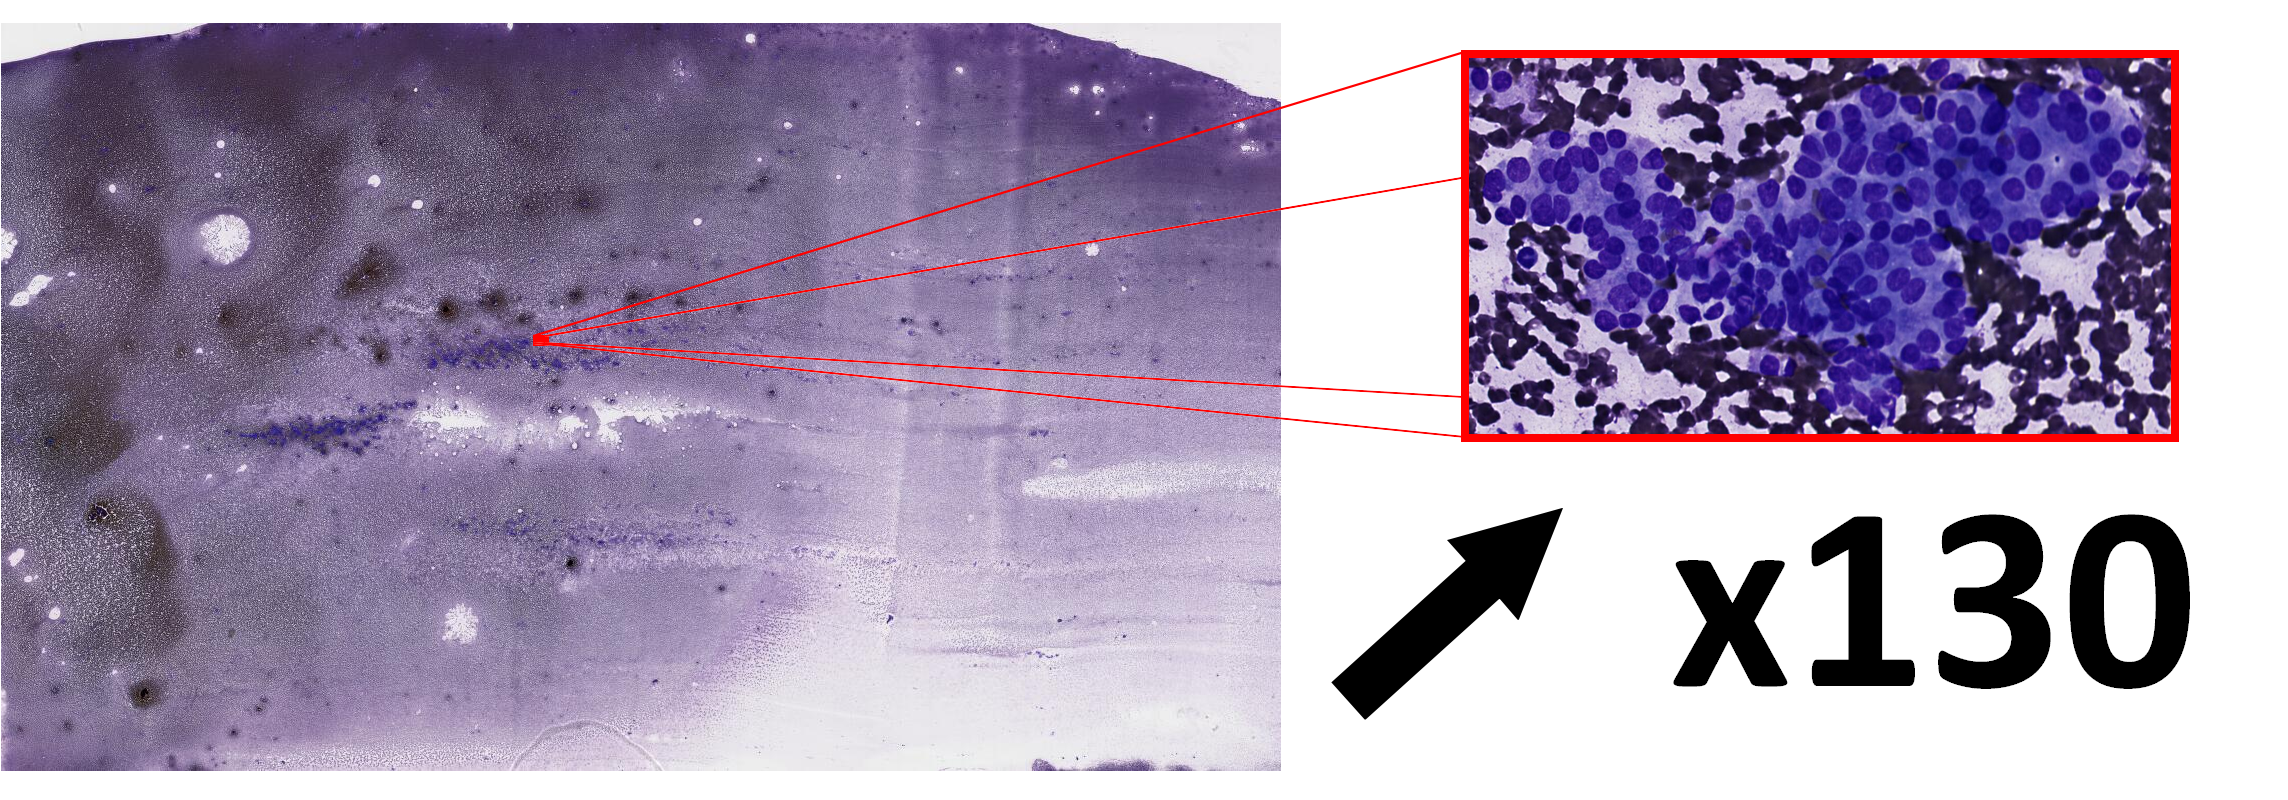
\includegraphics[height=80px]{images/whole-slide-dim.png}} \\
		\begin{multicols}{2}
		\centering
		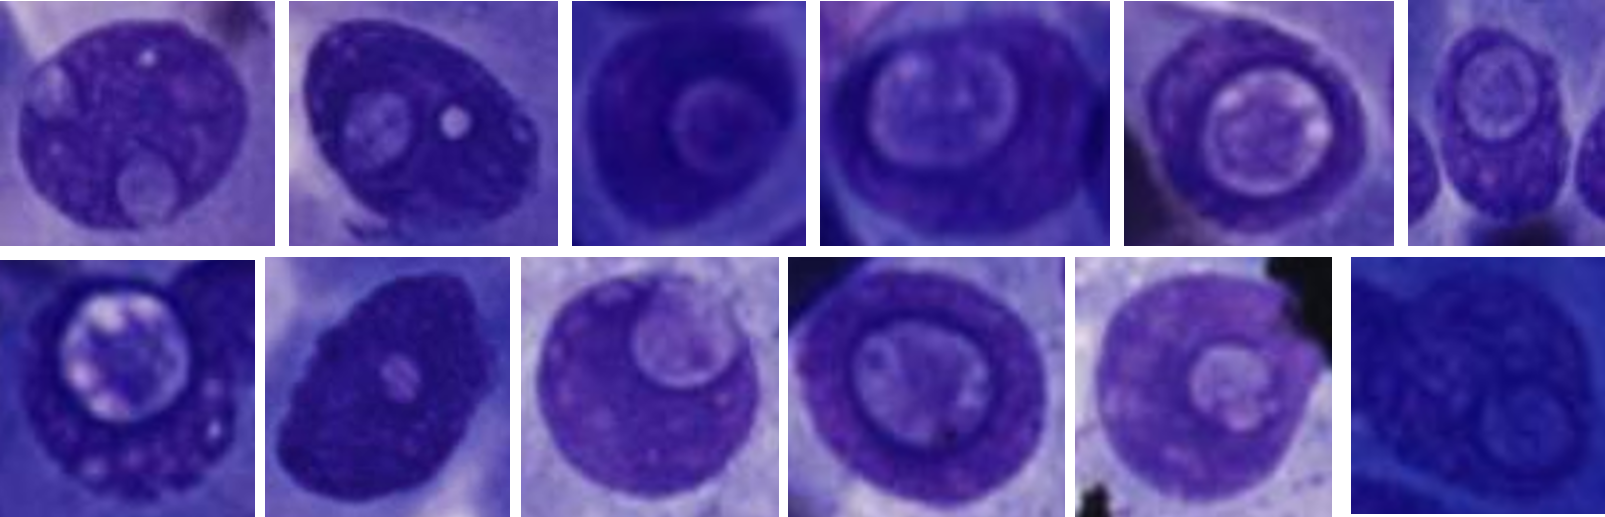
\includegraphics[height=40px]{thyroid/incl_centered.png}\\
		Malignant
		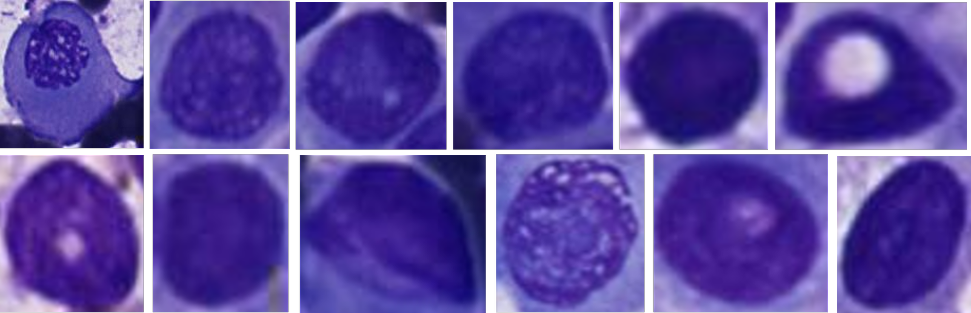
\includegraphics[height=40px]{thyroid/norm_centered.png}\\
		Benign
		\end{multicols}
	\end{figure}

	\vfill
\end{frame}


\begin{frame}{Objectives}
	\begin{center}
		\large
		Explore and develop new methods adapted to \textit{small data} problems.
	\end{center}
	
	\vfill
	Tracks and research questions: 
	\begin{enumerate}
		\item \textit{Interactive machine learning (iML)} : how to \textbf{integrate human operators to the learning process} in order to improve performances of ML methods?
		\item \textit{Transfer learning}: how to \textbf{leverage any available auxiliary data} for reaching the same goal ? 
	\end{enumerate}

\end{frame}
 
  
\begin{frame}{Typical machine learning}
	
	From ... 
	
	\begin{figure}[h]
		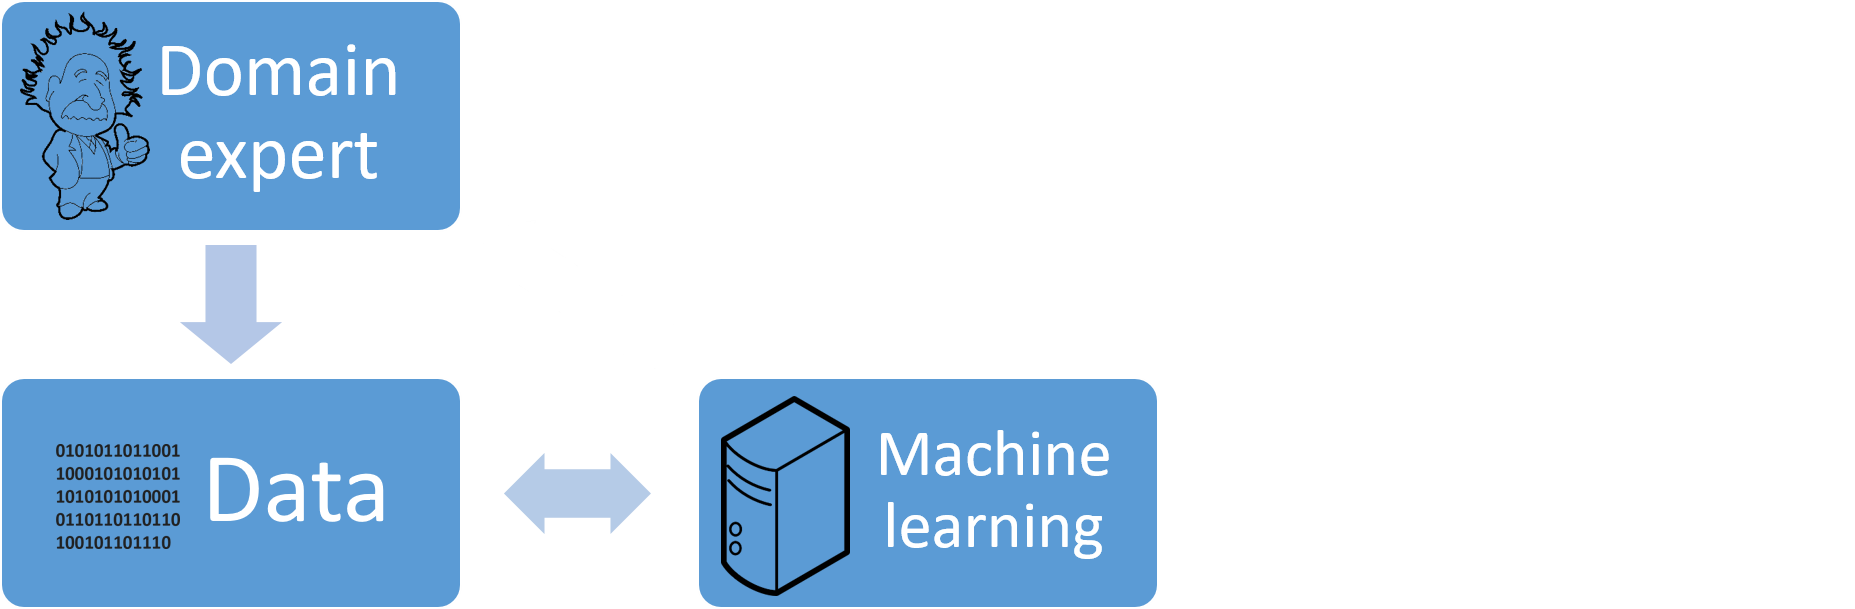
\includegraphics[height=160px]{images/ml_typical.png}
	\end{figure}
	

\end{frame}

\begin{frame}{Integrating human(s) and auxiliary data}
	
	To ... 
	
	\begin{figure}
		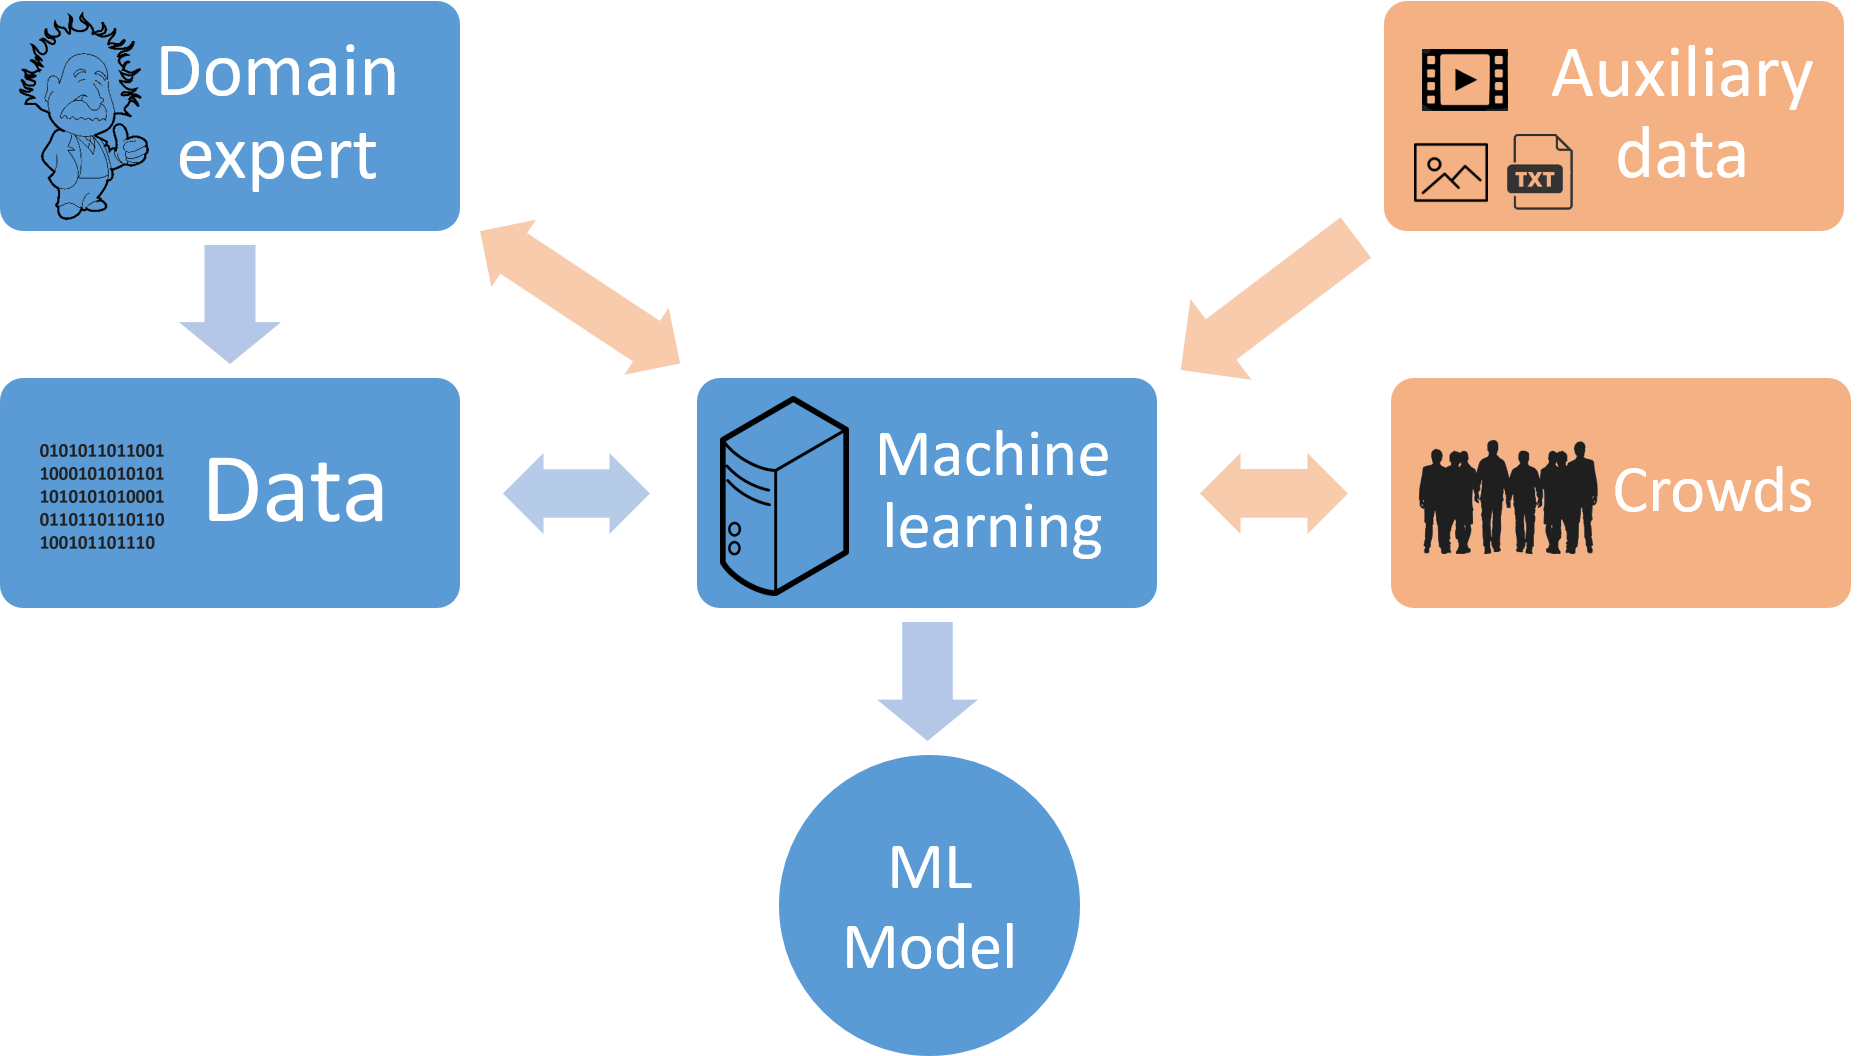
\includegraphics[height=160px]{images/ml_expert_crowds_aux_all.png}
	\end{figure}	
	
\end{frame}

\begin{frame}{Interactive machine learning}
	State of the art:
	\begin{itemize}
		\item Mostly \textbf{active learning} (i.e. smart example labelling)
		\item Few developments around richer forms of feedback
	\end{itemize}		
	\vfill
	Methodological challenges:
	\begin{itemize}
		\item How to \textbf{minimize the number of interactions} ? {\small(the method/system must \textit{ask the right questions})}
		\item How to \textbf{minimize time between each interaction} ? {\small(the method/system must \textit{be fast and reactive})}
		\item How to \textbf{integrate the feedback} to the learning process ?
	\end{itemize}

\end{frame}

\begin{frame}{Error labelling}
	\begin{figure}
		\center
		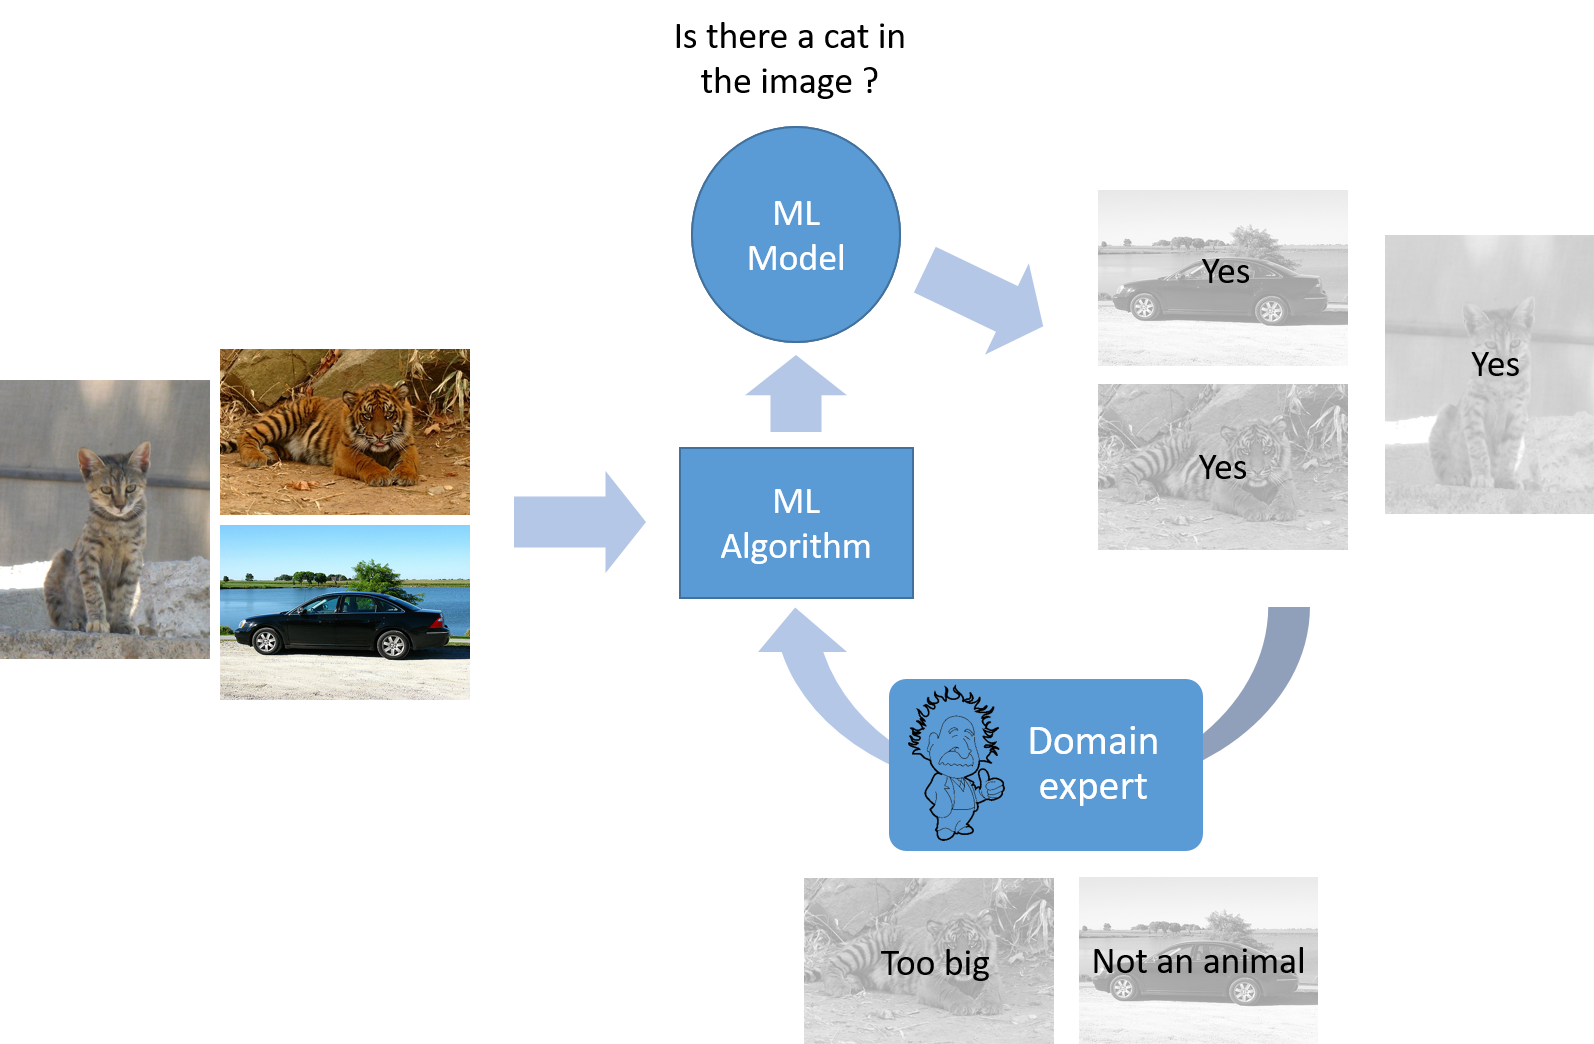
\includegraphics[height=200px]{images/error_labelling.png}
	\end{figure}
\end{frame}

\begin{frame}{A platform ready for user-interaction}
	
\includegraphics[height=1em]{images/cytomine_typo.png}, an open-source web platform will be used for collecting \textbf{feedback} from experts and from the crowds. \\  
	\vspace*{0.25cm}
	\hspace*{-0.75in}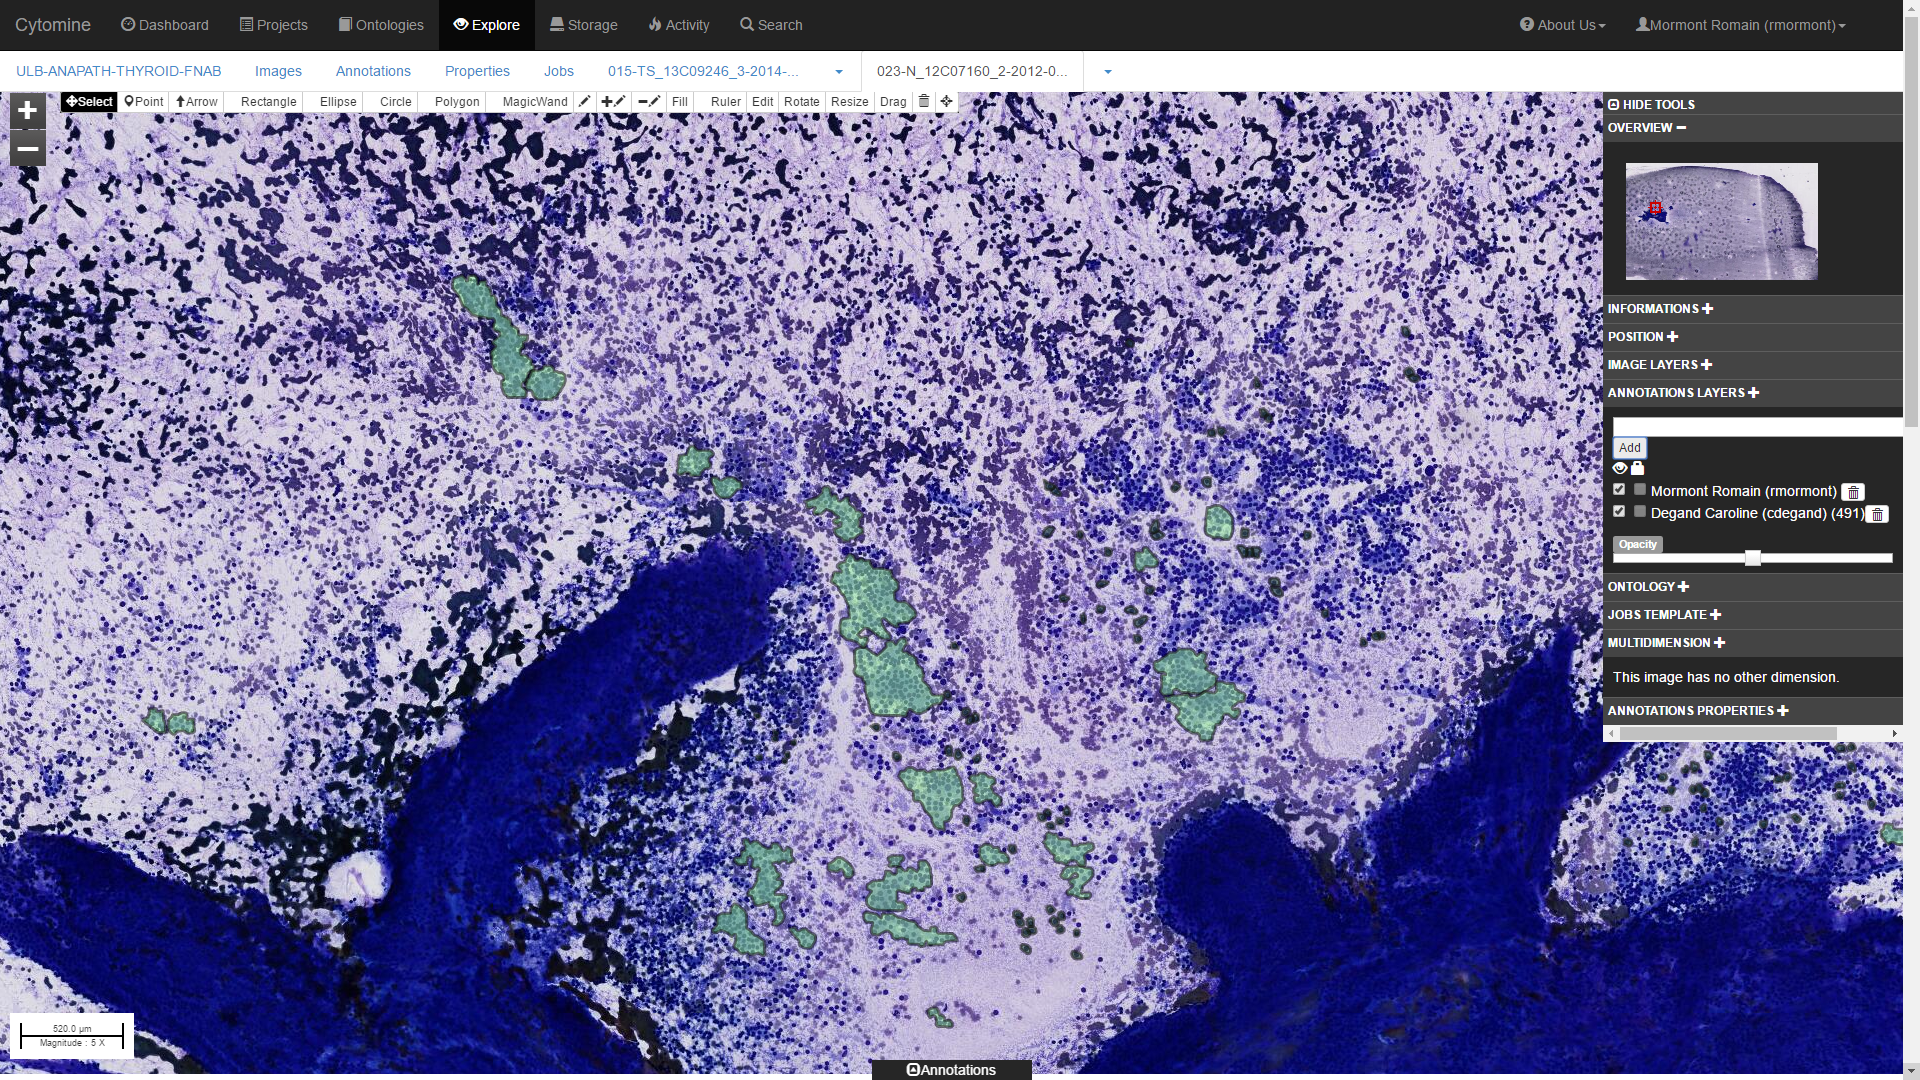
\includegraphics[width=400px]{images/cytomine.png}
\end{frame}



\begin{frame}
	\begin{center}
	
		Thank you for your attention! \\ 
		
	\end{center}
	\vfill
	\begin{figure}
		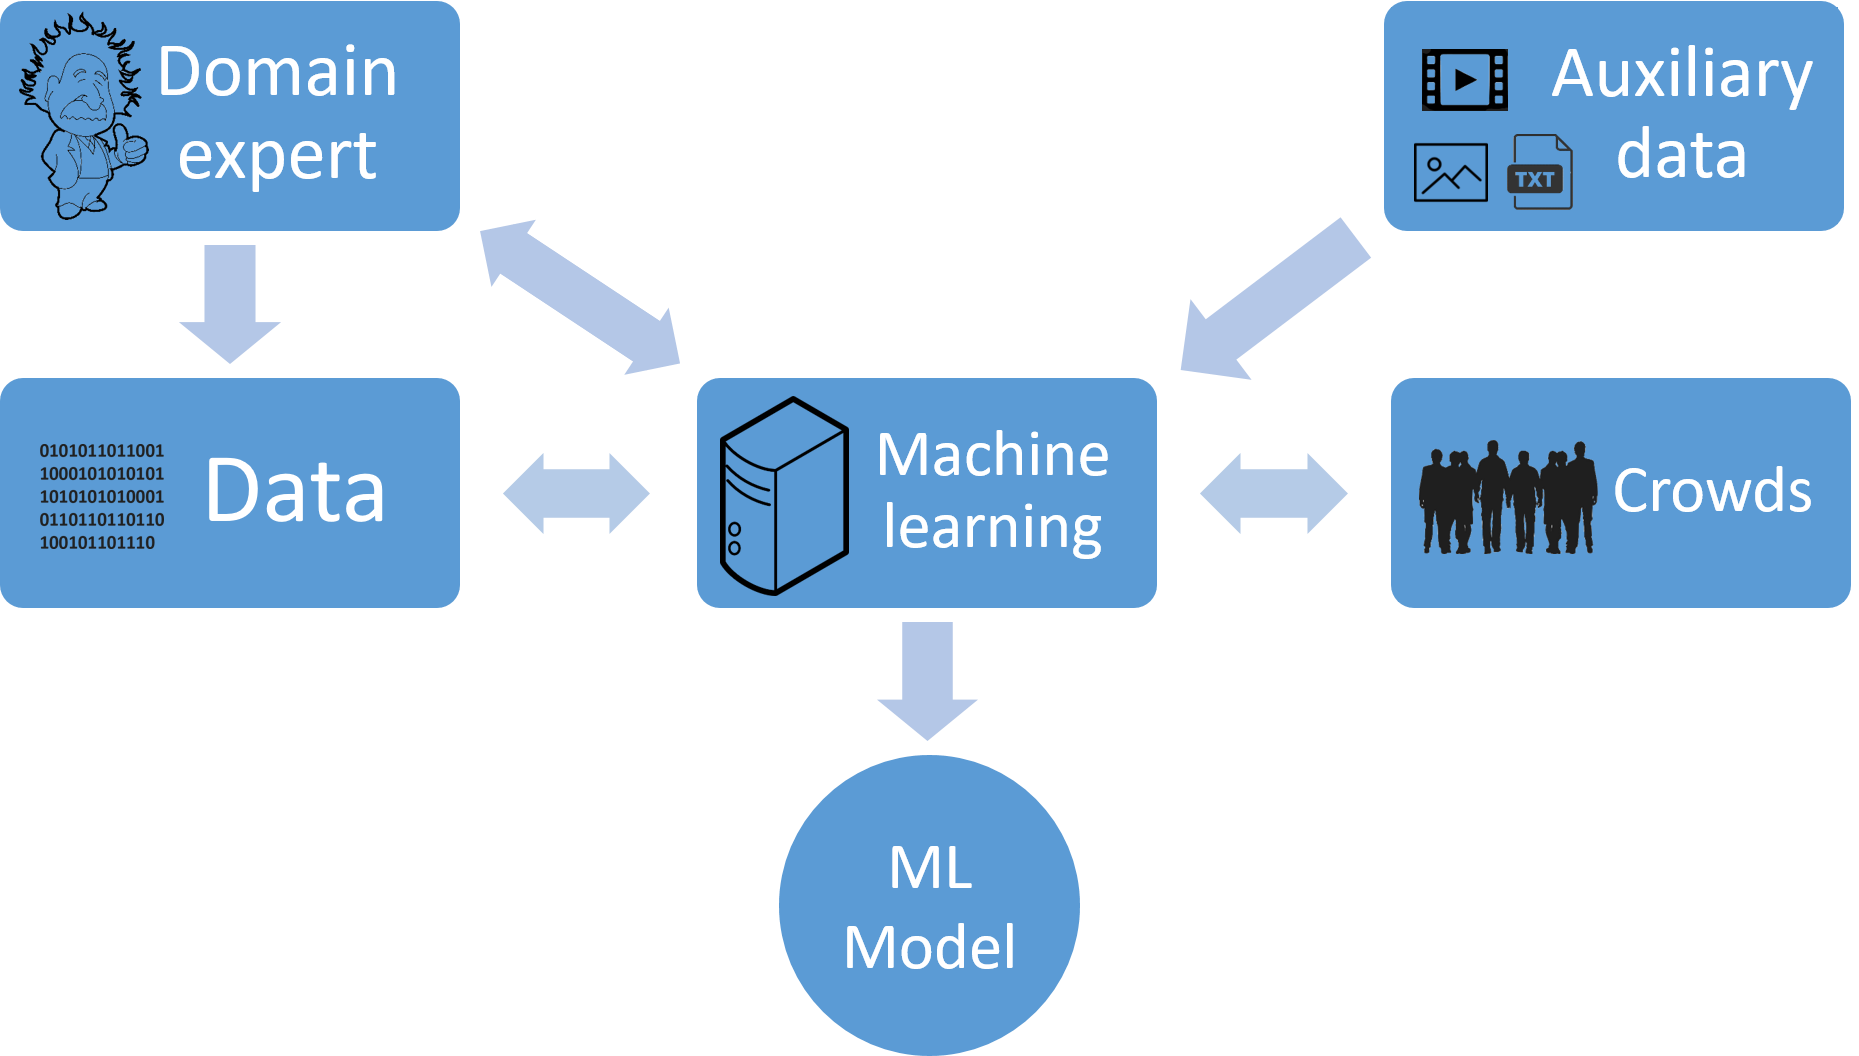
\includegraphics[height=175px]{images/ml_expert_crowds_aux_uni.png}
	\end{figure}
	\vfill
\end{frame}

\begin{frame}{Small data: illustration}
\begin{columns}
\begin{column}{0.48\textwidth}
	\footnotesize
	\center
		{\small	
		\textbf{Big data} \\
		ImageNet\footnotemark
		}
	\vfill
	\flushleft
		\textit{Dataset}: 
		\begin{itemize}
			\item 14M labelled images
			\item Enough data to learn inter- and intra-class variabilities
		\end{itemize}
		
		\begin{figure}[!h]
			\subfigure{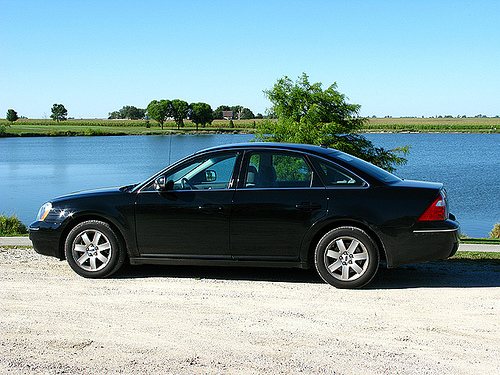
\includegraphics[height=25px]{imagenet/car.jpg}}
			\subfigure{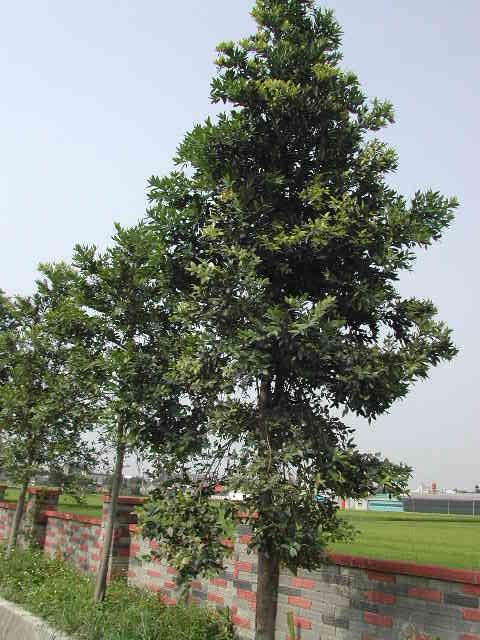
\includegraphics[height=25px]{imagenet/tree.jpg}}
			\subfigure{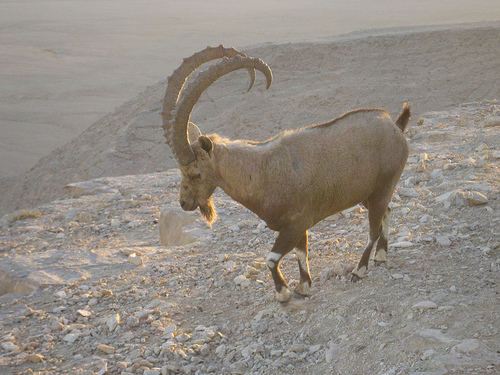
\includegraphics[height=25px]{imagenet/goat.jpg}}
			\subfigure{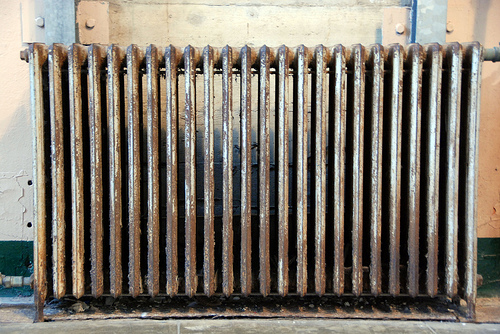
\includegraphics[height=25px]{imagenet/radiator.jpg}}\\
			\subfigure{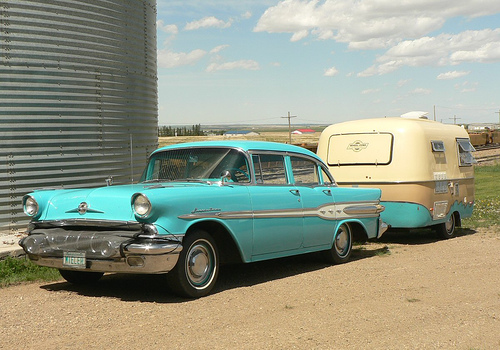
\includegraphics[height=25px]{imagenet/car2.jpg}}
			\subfigure{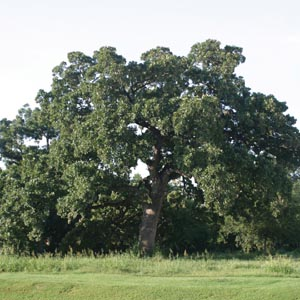
\includegraphics[height=25px]{imagenet/tree2.jpg}}
			\subfigure{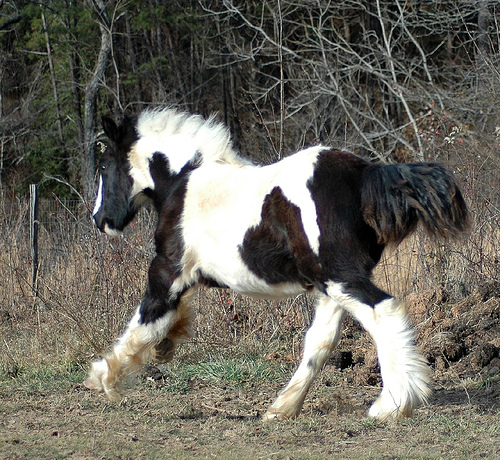
\includegraphics[height=25px]{imagenet/goat2.jpg}}
			\subfigure{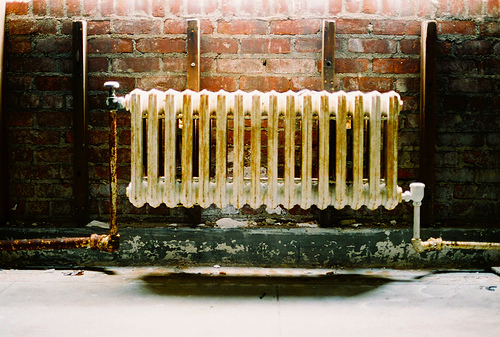
\includegraphics[height=25px]{imagenet/radiator2.jpg}}
			\caption{Typical images from ImageNet}
		\end{figure}
\end{column}
\hfill
\begin{column}{0.5\textwidth}  
	\footnotesize
	\center
		{\small		
		\textbf{Small data} \\
		Thyroid nodule malignancy
		}
	\vfill
	\flushleft
		\textit{Dataset}:
		\begin{itemize}
			\item 6K labelled images
			\item Most important objects (i.e. malignant) are rare
		\end{itemize}
	
		\begin{figure}[!h]
		\subfigure[Healthy]{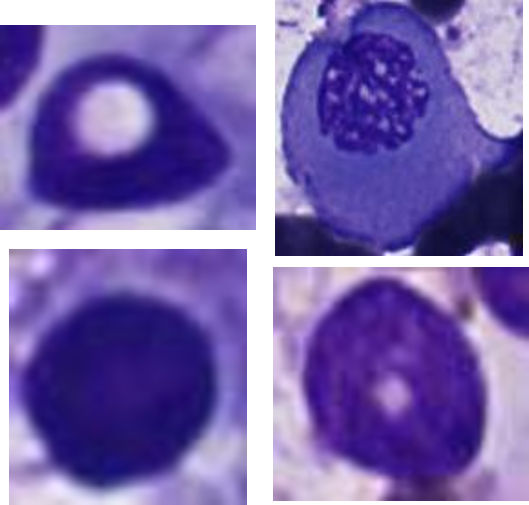
\includegraphics[scale=0.12]{thyroid/norm.png}}
		\hfill
		\subfigure[Malignant]{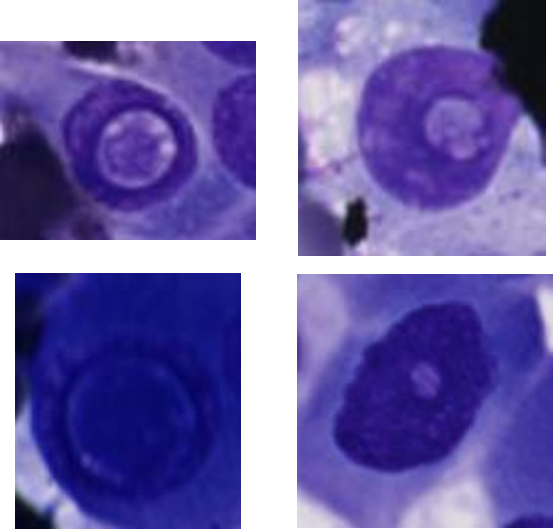
\includegraphics[scale=0.12]{thyroid/incl.png}}
		\end{figure}
\end{column}
\end{columns}
\footnotetext[1]{Deng \& al. \textit{ImageNet: A Large-Scale Hierarchical Image Database}. In CVPR09, 2009.}
\end{frame}


\begin{frame}{Work calendar}
	\footnotesize
	\begin{table}
	\hspace*{-0.5cm}
	\setlength\tabcolsep{3pt} % default value: 6pt
	\begin{tabular}{|c|r|ccc|cccccccccccc|cccccccccccc|cccccccccccc|}
		\hline
		& & \multicolumn{3}{c|}{2016} & \multicolumn{12}{c|}{2017} & \multicolumn{12}{c|}{2018}  & \multicolumn{12}{c|}{2019}  \\
		\hline	
		& & \multicolumn{3}{c|}{T4} & \multicolumn{3}{c|}{T1} & \multicolumn{3}{c|}{T2} & \multicolumn{3}{c|}{T3} & \multicolumn{3}{c|}{T4} & \multicolumn{3}{c|}{T1} & \multicolumn{3}{c|}{T2} & \multicolumn{3}{c|}{T3} & \multicolumn{3}{c|}{T4}  & \multicolumn{3}{c|}{T1} & \multicolumn{3}{c|}{T2} & \multicolumn{3}{c|}{T3} & \multicolumn{3}{c|}{T4}\\ 
		\hline
		& Setup & \cellcolor{black} & \cellcolor{black} & \cellcolor{black} & \cellcolor{black} & \cellcolor{black} & & & & & & & & & & & & & & & & & & & & & & & & & & & & & & & & & & \\
		\hdashline
		 \parbox[t]{2mm}{\multirow{3}{*}{\rotatebox[origin=c]{90}{\tiny  Interactive}}} & Active learning & & & & & & \cellcolor{black} & \cellcolor{black} & \cellcolor{black} & \cellcolor{black} & & & & & & & & & & & & & & & & & & & & & & & & & & & & & &\\
		& Error labelling & & & & & & & & & & \cellcolor{black} & \cellcolor{black} & \cellcolor{black} & \cellcolor{black} & \cellcolor{black} & \cellcolor{black} & & & & & & & & & & & & & & & & & & & & & & & & \\
		& Feature evaluat. & & & & & & & & & & & & & & & & \cellcolor{black} & \cellcolor{black} & \cellcolor{black} & \cellcolor{black} & \cellcolor{black} & \cellcolor{black} & & & & & & & & & & & & & & & & & & \\
		\hdashline
		 \parbox[t]{2mm}{\multirow{3}{*}{\rotatebox[origin=c]{90}{\tiny Aux. data}}} & Survey \& setup & & & & & & & & & & & & & & & & & & & & & & \cellcolor{black} & & & & & & & & & & & & & & & & & \\
		& Imprecise data & & & & & & & & & & & & & & & & & & & & & & & \cellcolor{black} & \cellcolor{black} & \cellcolor{black} & \cellcolor{black} & \cellcolor{black} & \cellcolor{black} & \cellcolor{black} & & & & & & & & & & \\
		& Multi-modal & & & & & & & & & & & & & & & & & & & & & & & & & & & & & & \cellcolor{black} & \cellcolor{black} & \cellcolor{black} & \cellcolor{black} & \cellcolor{black} & \cellcolor{black} & & & & \\
		\hdashline
		& Extension 
		& & & & & & & & & & & & & & & & & & & & & & & & & & & & & & & & & & & & \cellcolor{black} & \cellcolor{black} & \cellcolor{black} & \cellcolor{black} \\
		\hline 
	\end{tabular}


\vfill

	\begin{tabular}{|c|r|cccccccccccc|}
		\hline
		& & \multicolumn{12}{c|}{2020}  \\
		\hline	
		& & \multicolumn{3}{c|}{T1} & \multicolumn{3}{c|}{T2} & \multicolumn{3}{c|}{T3} & \multicolumn{3}{c|}{T4} \\ 
		\hline
		& Extension & \cellcolor{black} & \cellcolor{black} & & & & & & & & &  & \\
		& Writing & & & \cellcolor{black} & \cellcolor{black} & \cellcolor{black} & \cellcolor{black} & \cellcolor{black} & \cellcolor{black} & & & & \\
		\hline 
	\end{tabular}


	\end{table}
\end{frame}


\begin{frame}{Master thesis}	
	\begin{center}
		\textbf{A workflow for large-scale computer-aided cytology and its applications.}
	\end{center}		
	\begin{figure}
		\center
		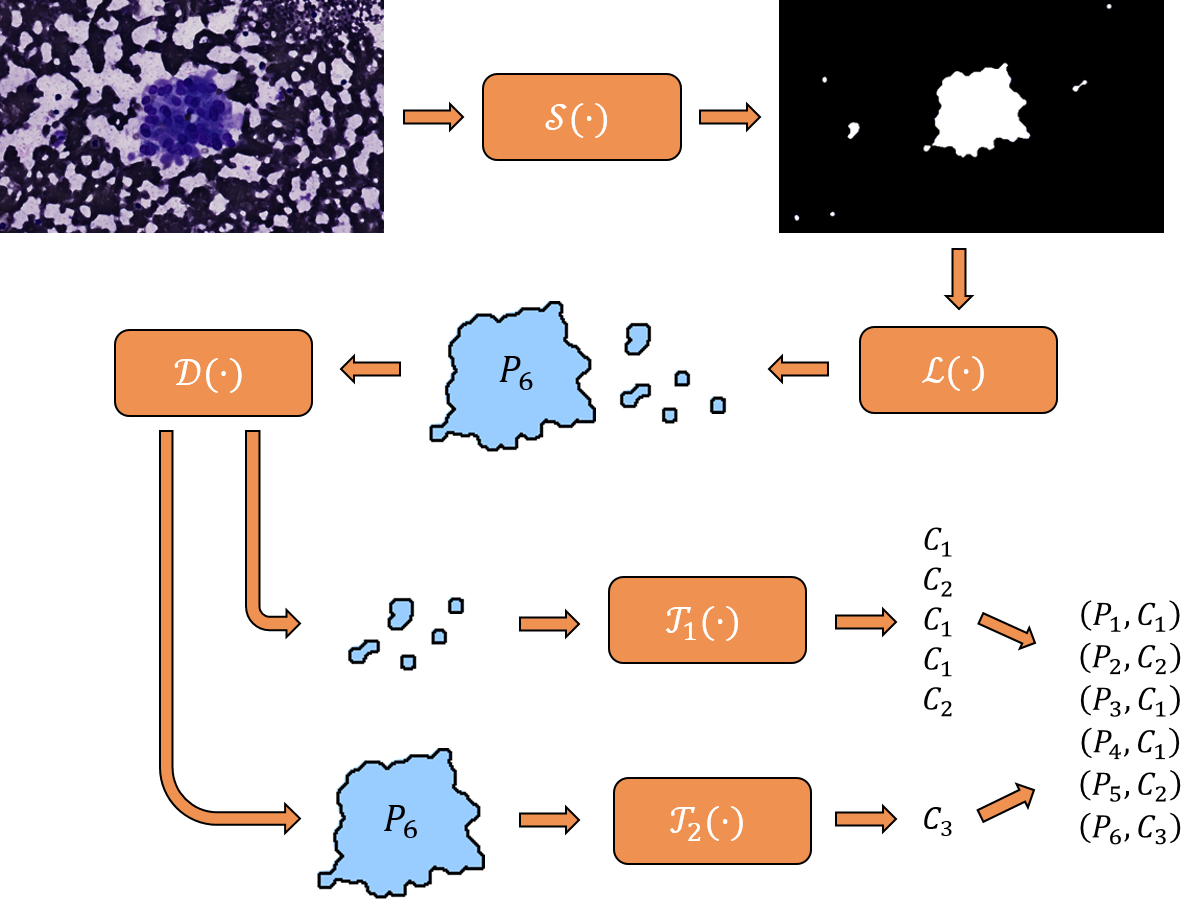
\includegraphics[height=150px]{images/workflow_illustration.png}
	\end{figure}	
\end{frame}

\begin{frame}{Question 2: transfer learning ?}
	
	Methodological challenges:
	\begin{itemize}
		\item \textbf{What information should be transferred} to improve performances and avoid negative transfer? 
		\item \textbf{How to integrate this information} into the methods ? 
	\end{itemize}
	
	\vfill
	Focus on two settings:
	
	\begin{itemize}
		\item Imprecise measurements 
		\item Multi-modal images
	\end{itemize}

	\begin{figure}
		\center
		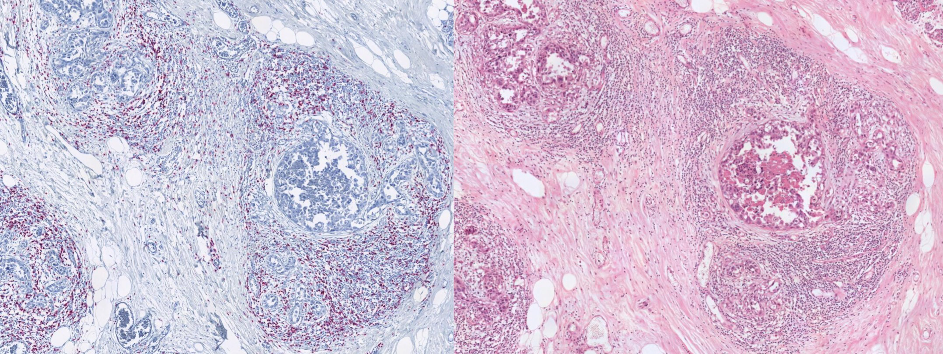
\includegraphics[height=113px]{images/multimodal.png}
	\end{figure}	
	
	
\end{frame}


\begin{frame}{Feature evaluation}
	\begin{figure}
		\center
		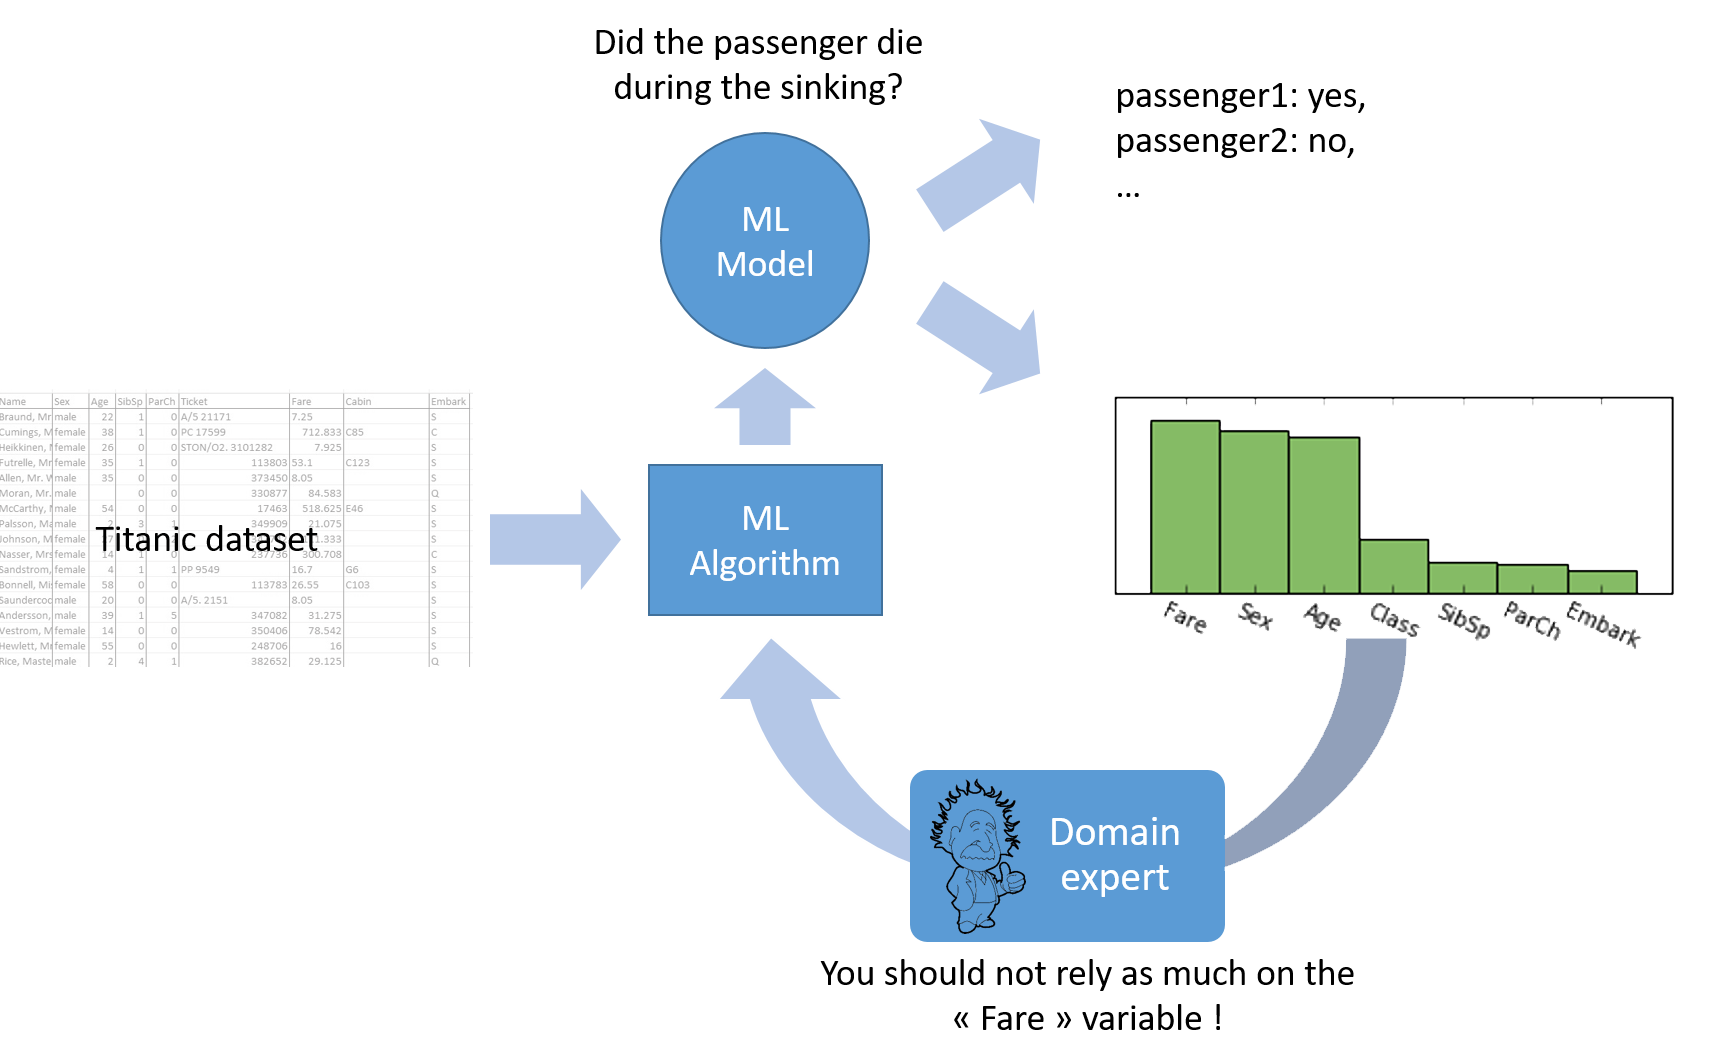
\includegraphics[height=200px]{images/feature_evaluation.png}
	\end{figure}
\end{frame}

\end{document}
